\begin{figure}[H]
	\centering
	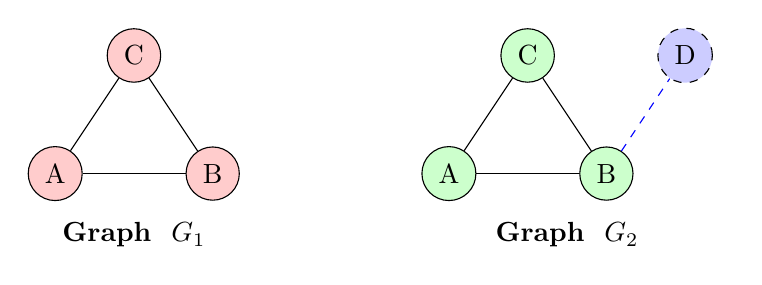
\begin{tikzpicture}
		% Graph G1
		\node[circle, draw, fill=red!20] (A1) at (0,0) {A};
		\node[circle, draw, fill=red!20] (B1) at (2,0) {B};
		\node[circle, draw, fill=red!20] (C1) at (1,1.5) {C};
		\draw (A1) -- (B1);
		\draw (A1) -- (C1);
		\draw (B1) -- (C1);
		\node[align=center, below] at (1, -0.5) {\textbf{Graph } $G_1$};
		
		% Graph G2
		\node[circle, draw, fill=green!20] (A2) at (5,0) {A};
		\node[circle, draw, fill=green!20] (B2) at (7,0) {B};
		\node[circle, draw, fill=green!20] (C2) at (6,1.5) {C};
		\node[circle, draw, fill=blue!20, dashed] (D2) at (8,1.5) {D};
		\draw (A2) -- (B2);
		\draw (A2) -- (C2);
		\draw (B2) -- (C2);
		\draw[dashed, blue] (B2) -- (D2);
		\node[align=center, below] at (6.5, -0.5) {\textbf{Graph } $G_2$};
		
		% New vertex and edge addition
		\node[align=center, above] at (8.5, 1.5) {};
		\node[align=center, right] at (7.5, 0.75) {};
		
	\end{tikzpicture}
	\caption{Graph Edit Distance: Transforming $G_1$ to $G_2$ by adding vertex D and edge (B,D).}
	\label{fig:ged-graphs}
\end{figure}
